% This is the now Chapter 6

This comprehensive evaluation presents compelling evidence for the effectiveness of our proposed multimodal pedagogical assessment framework, demonstrating significant advancements in automated teaching evaluation through integrated data analysis. Our research addresses the critical need for objective, scalable assessment tools in educational environments by combining visual behavioral patterns, audio-prosodic features, and linguistic discourse analysis into a unified predictive model. 

The experimental results reveal that multimodal integration achieves 71.33\% accuracy using Logistic Regression, representing a substantial 4.33\% improvement over the best individual modality (linguistic features at 67.0\%), while maintaining superior cross-validation stability with reduced performance variance. These findings align directly with our primary research objectives of developing a comprehensive assessment framework that captures the multifaceted nature of effective teaching, providing actionable feedback mechanisms for educators, and establishing a foundation for scalable deployment in diverse educational contexts.

The demonstrated synergistic effects between modalities, enhanced model stability, and practical applicability of our approach validate the central hypothesis that integrated multimodal analysis significantly enhances pedagogical assessment accuracy and reliability. Furthermore, the results establish a robust empirical foundation for future developments in automated educational quality assurance systems, positioning our methodology as a viable solution for large-scale implementation in institutional settings where traditional assessment methods may be limited by subjectivity, scalability constraints, or resource availability.

This section presents the comprehensive evaluation of the proposed multimodal approach for pedagogical assessment. The analysis compares the performance of individual modalities (visual, audio, and linguistic) against the combined multimodal approach using two machine learning algorithms: Logistic Regression and Support Vector Machine (SVM).

The experimental results demonstrate a clear superiority of the multimodal approach over individual modality-based assessments. Table~\ref{tab:performance_table} presents the comprehensive performance metrics across all tested configurations.


\begin{figure}[H]
    \centering
    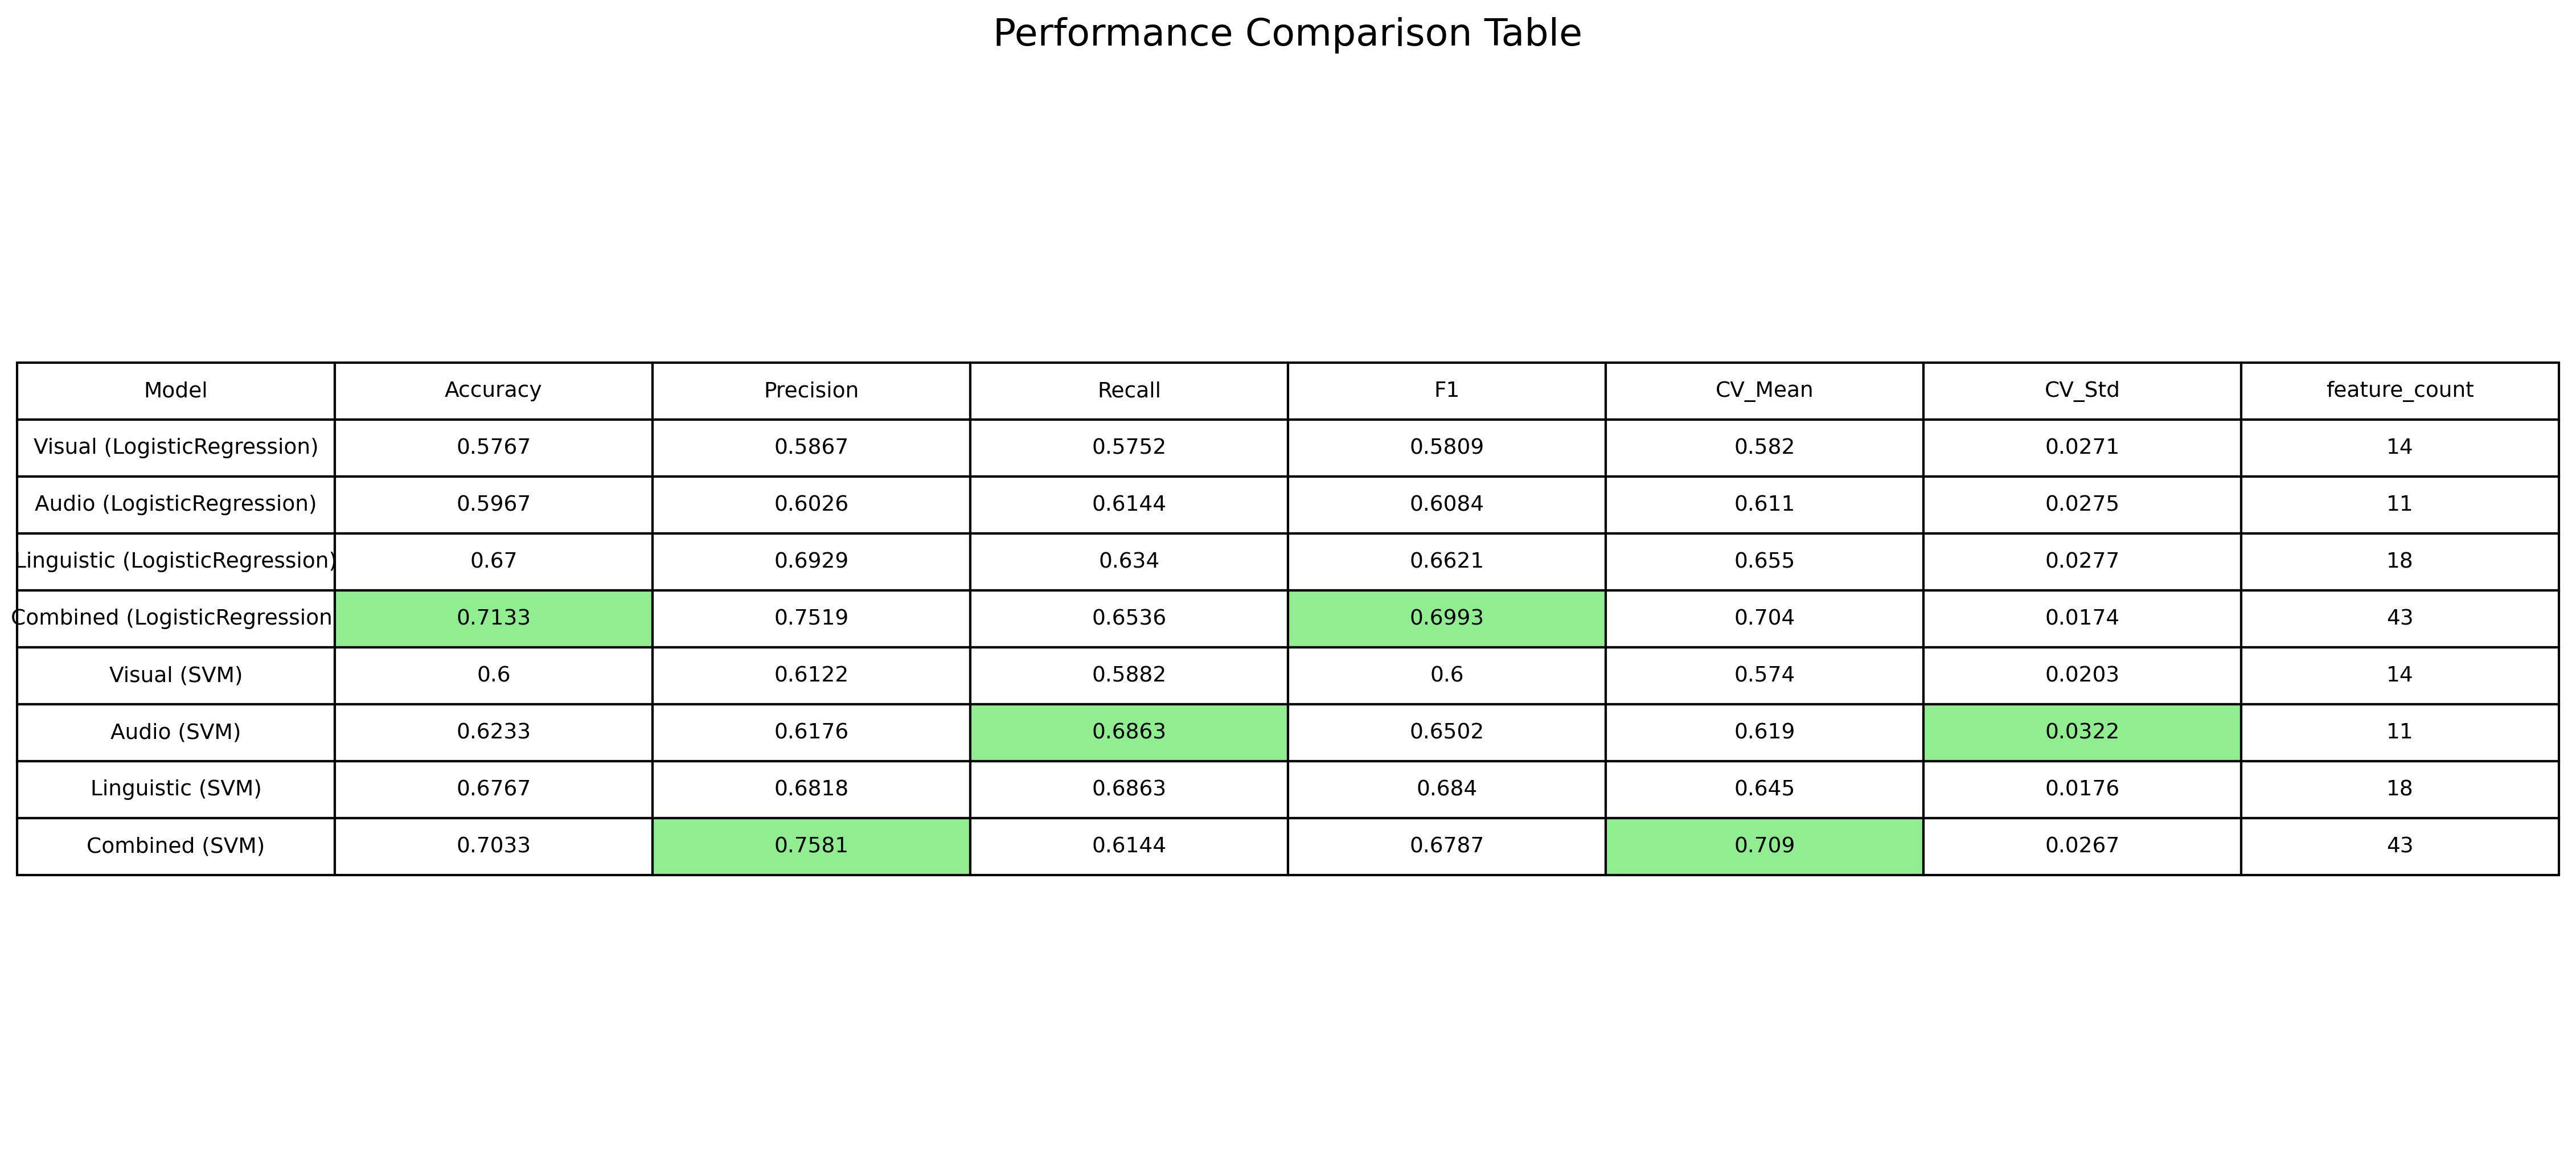
\includegraphics[width=0.9\textwidth]{sections/performance_table.jpg}
    \caption{Comprehensive Performance Comparison Table showing accuracy, precision, recall, F1-score, cross-validation means and standard deviations across all modality combinations and algorithms.}
    \label{fig:performance_table}
\end{figure}

The combined multimodal approach achieved the highest accuracy of 71.33\% using Logistic Regression, representing a substantial improvement over individual modalities. This finding strongly supports the central thesis that integrating multiple data sources provides a more comprehensive and accurate assessment of pedagogical outcomes.

\subsection{Individual Modality Analysis}

\subsubsection{Visual Features Performance}

Visual features encompassed teacher movement patterns, gesture frequency, classroom coverage, and facial expressions, demonstrating moderate predictive capability in pedagogical assessment. The visual modality achieved \textbf{57.67\%} accuracy with Logistic Regression and \textbf{60.0\%} accuracy with SVM, representing the lowest performance among individual modalities.

Despite this relative underperformance, several visual indicators emerged as meaningful contributors to pedagogical effectiveness assessment. These included classroom coverage patterns that reflect teacher mobility and engagement with different student zones, frontal stance duration indicating direct interaction time with students, gesture frequency representing pedagogical expressiveness and emphasis, and spatial consistency measuring structured movement patterns that support organized content delivery. While visual features alone showed limitations in predictive accuracy, their integration with other modalities proved essential for comprehensive assessment, as demonstrated in subsequent multimodal results.

\subsubsection{Audio Features Performance}

Audio features demonstrated solid predictive performance through prosodic analysis and vocal pattern recognition, achieving \textbf{59.67\%} accuracy with Logistic Regression and \textbf{62.33\%} accuracy with SVM. The audio modality captured essential elements of effective pedagogical delivery including pitch variability that signals teacher engagement and emphasis during critical concepts, speech rate consistency that indicates controlled content pacing and student comprehension awareness, strategic pause utilization that demonstrates thoughtful discourse structuring and allows processing time, and vocal intensity modulation that reinforces key pedagogical points through natural emphasis patterns.

These prosodic characteristics proved particularly valuable when combined with other modalities, as vocal delivery often reinforces visual gestures and supports linguistic content structuring in effective teaching scenarios. The moderate performance of audio features alone suggests that while vocal patterns contribute meaningfully to pedagogical assessment, they achieve optimal effectiveness when integrated with complementary visual and linguistic modalities.

\subsubsection{Linguistic Features Performance}

Linguistic features emerged as the most predictive individual modality, achieving \textbf{67.0\%} accuracy with Logistic Regression and \textbf{67.67\%} accuracy with SVM. This superior performance highlights the fundamental importance of discourse quality in pedagogical effectiveness assessment.

The linguistic analysis captured essential elements of effective teaching delivery including lexical diversity metrics that quantify vocabulary richness and adaptability to student comprehension levels, interactive question ratios that measure facilitated student engagement and participation, strategic deployment of examples and summaries indicating structured content scaffolding, and discourse complexity levels that assess cognitive engagement depth through Bloom's taxonomy frameworks.

The consistently strong performance across both algorithms establishes linguistic features as the most reliable foundation for pedagogical assessment, reflecting the central role of verbal communication in educational content delivery and classroom relationship establishment.

\subsection{Multimodal Integration Results}

\begin{figure}[H]
    \centering
    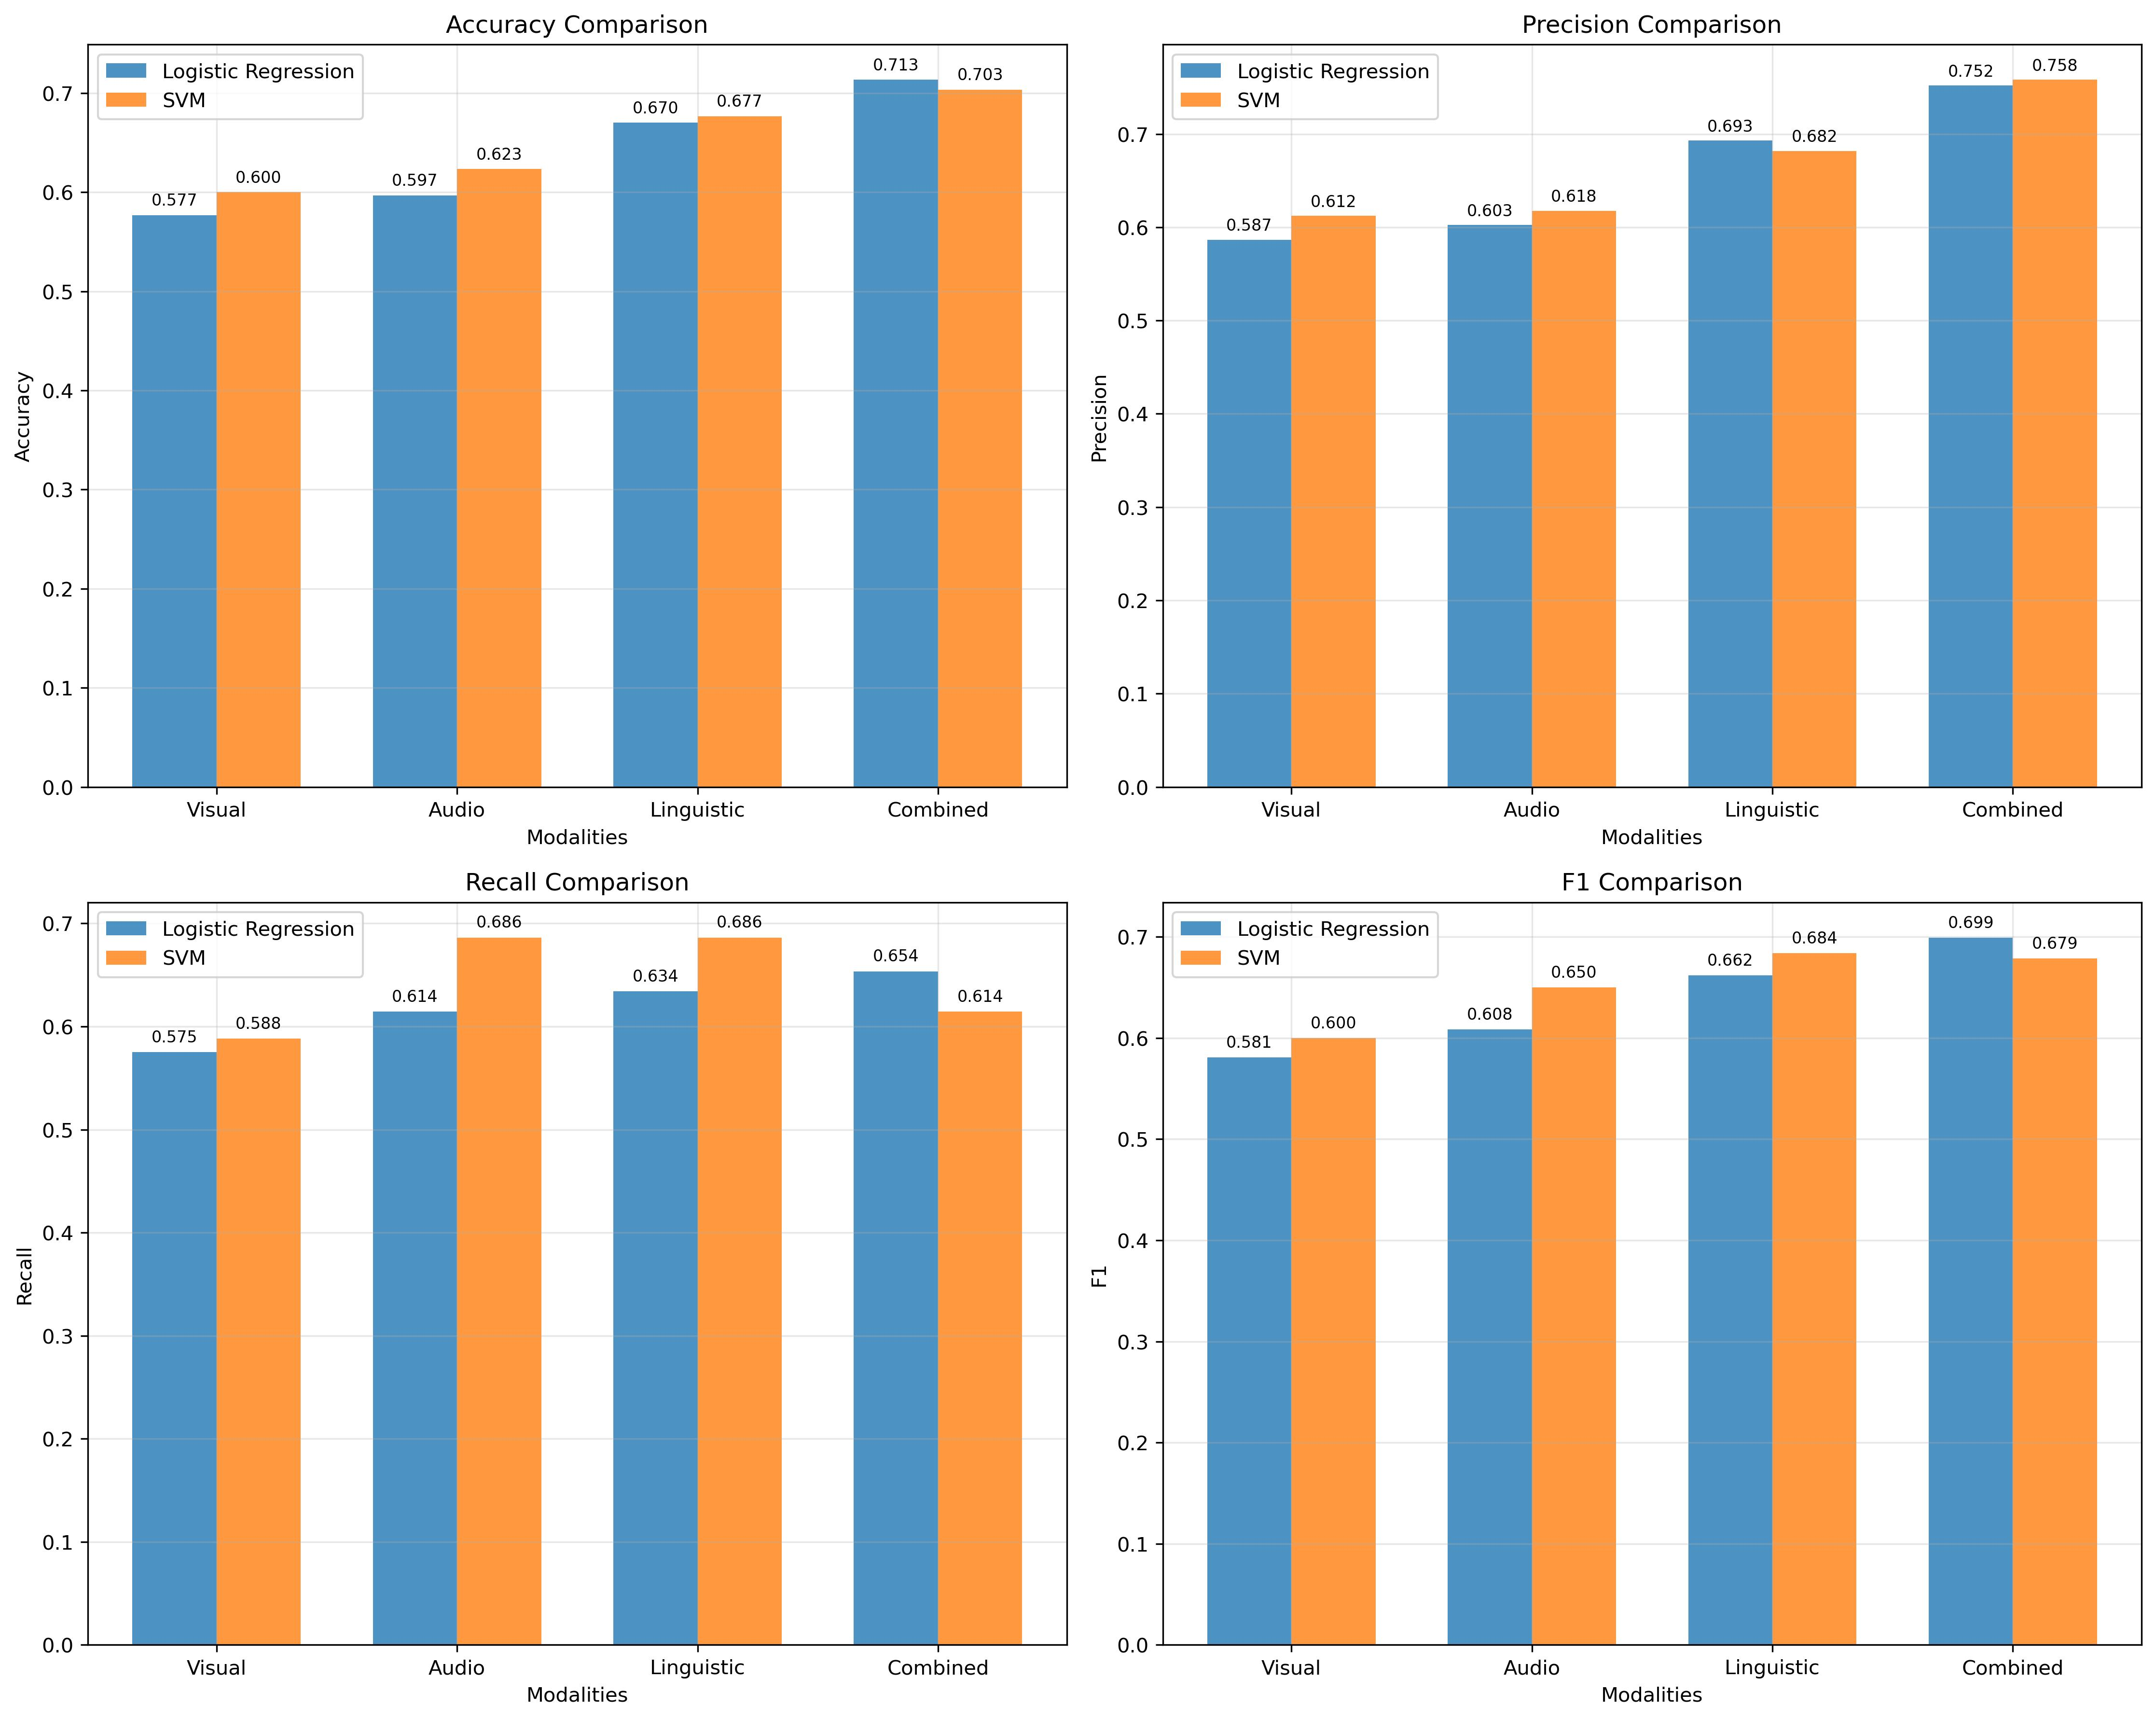
\includegraphics[width=\textwidth]{sections/performance_comparison.jpg}
    \caption{Performance comparison across all modalities and algorithms. The combined multimodal approach consistently outperforms individual modalities across all evaluation metrics (accuracy, precision, recall, and F1-score).}
    \label{fig:performance_comparison}
\end{figure}

The integration of all three modalities resulted in significant performance improvements. The combined approach achieved 71.33\% accuracy with Logistic Regression and 70.33\% accuracy with SVM, representing improvements of 4.33\% and 2.66\% respectively over the best individual modality (linguistic).

These improvements can be attributed to the complementary nature of different modalities:
\begin{itemize}
    \item \textbf{Visual-Audio Synergy:} Non-verbal cues complementing vocal emphasis patterns
    \item \textbf{Audio-Linguistic Correlation:} Prosodic features reinforcing discourse quality measures
    \item \textbf{Visual-Linguistic Alignment:} Physical positioning supporting pedagogical discourse strategies
\end{itemize}

\subsection{Cross-Validation Analysis}

\begin{figure}[H]
    \centering
    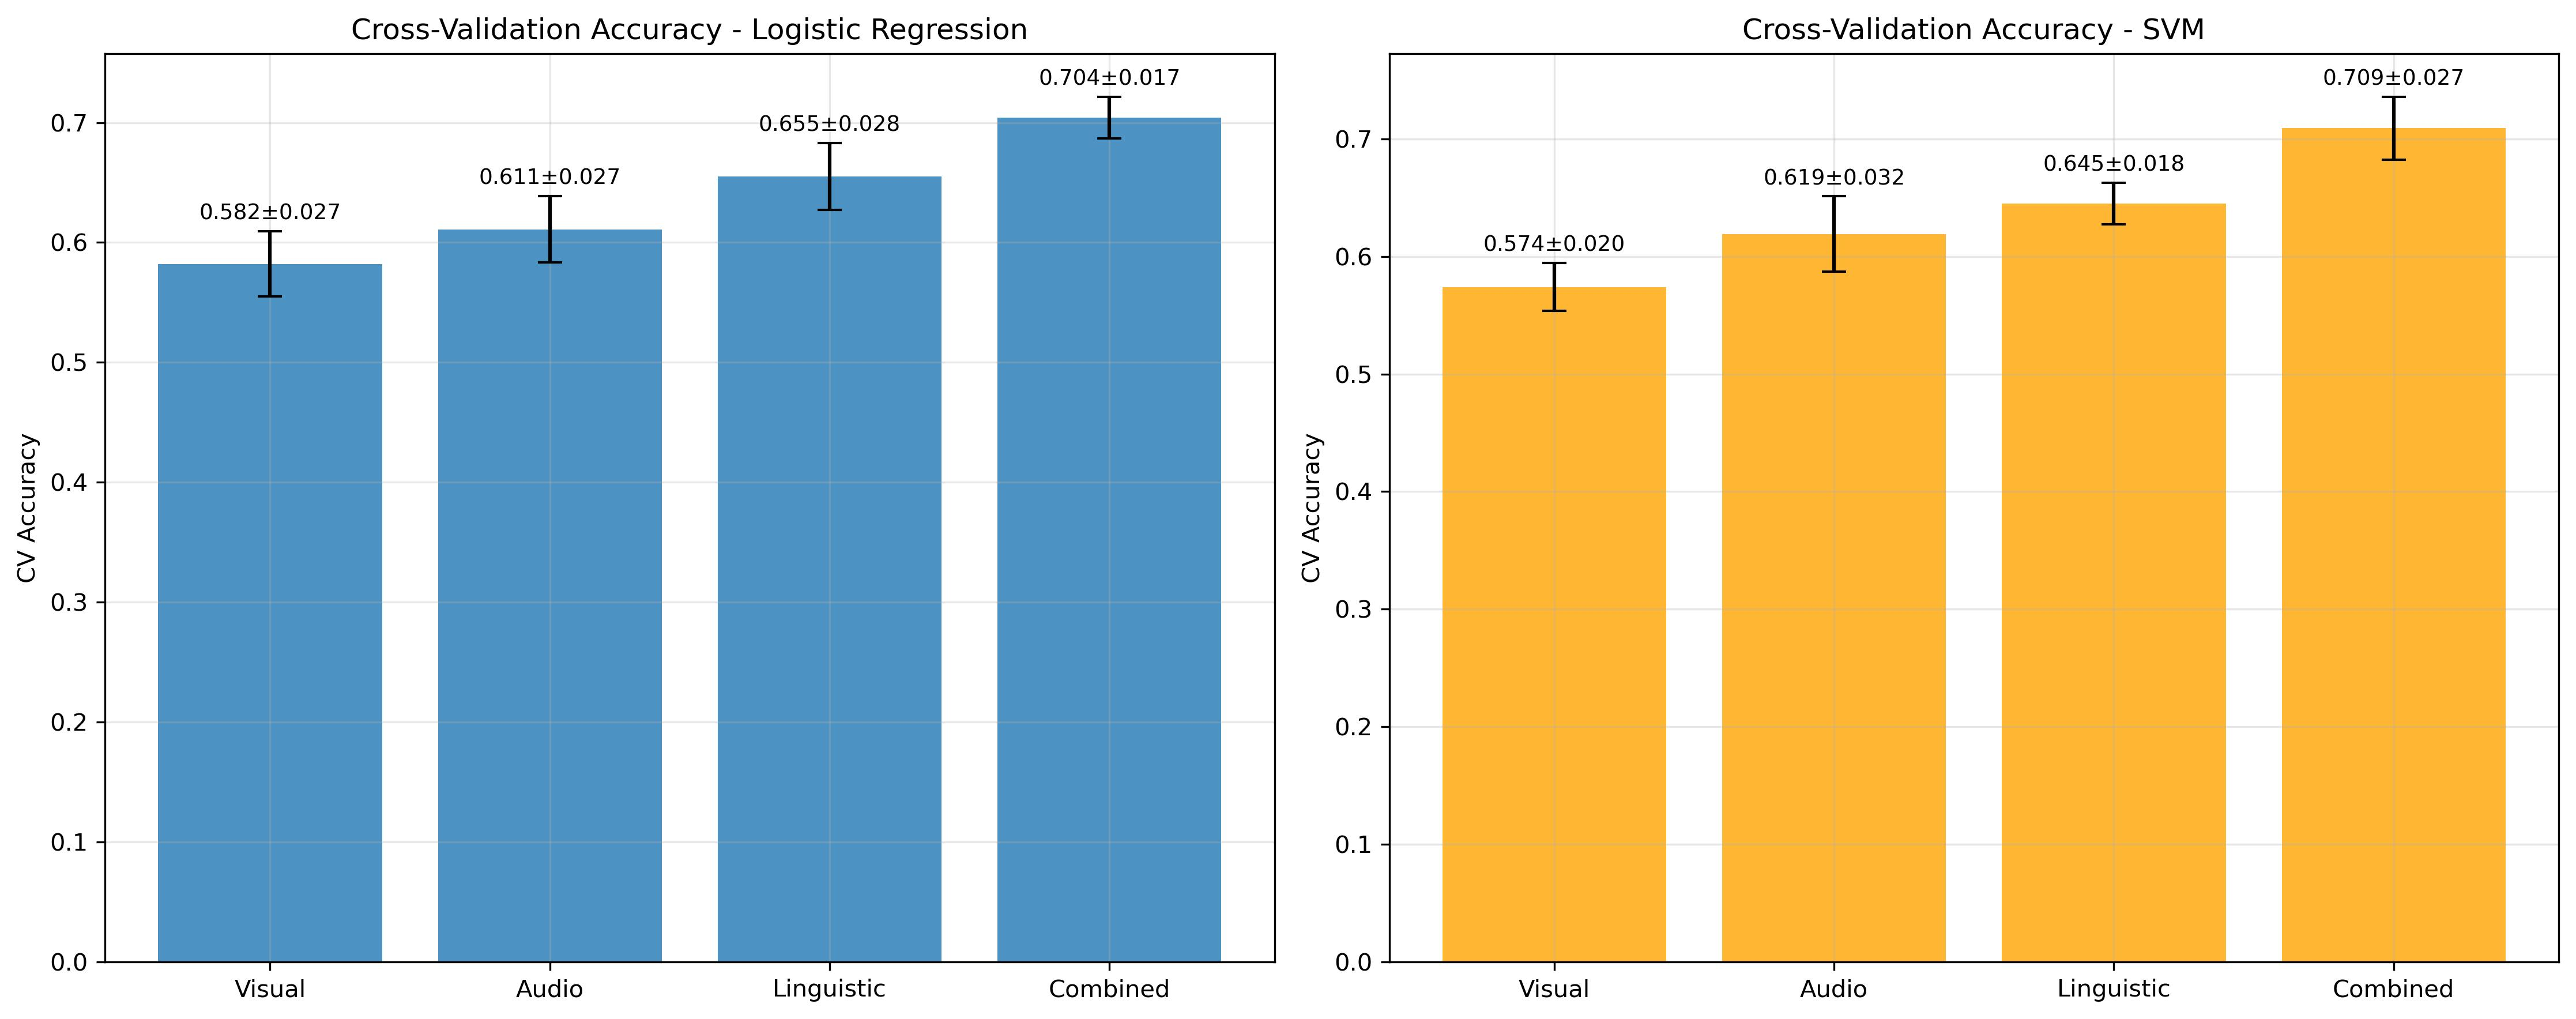
\includegraphics[width=\textwidth]{sections/cross_validation_comparison.jpg}
    \caption{Cross-validation accuracy results with error bars showing standard deviation. The multimodal approach demonstrates superior performance stability across both algorithms with reduced variance.}
    \label{fig:cross_validation}
\end{figure}

Cross-validation results provide robust evidence of the multimodal approach's superiority and stability. The combined approach achieved a mean cross-validation accuracy of \textbf{70.4\% (±1.74\%)} for Logistic Regression and \textbf{70.9\% (±2.67\%)} for SVM, with notably lower variance compared to individual modalities. The reduced standard deviation in the multimodal approach indicates enhanced model stability across different data splits, reduced overfitting through feature diversification, and more consistent performance across varying teaching contexts. This stability is particularly crucial for pedagogical assessment systems, where consistent evaluation standards are essential for maintaining educational quality and providing reliable feedback to instructors across diverse teaching scenarios.

\subsection{Feature Scaling and Model Performance}

\begin{figure}[H]
    \centering
    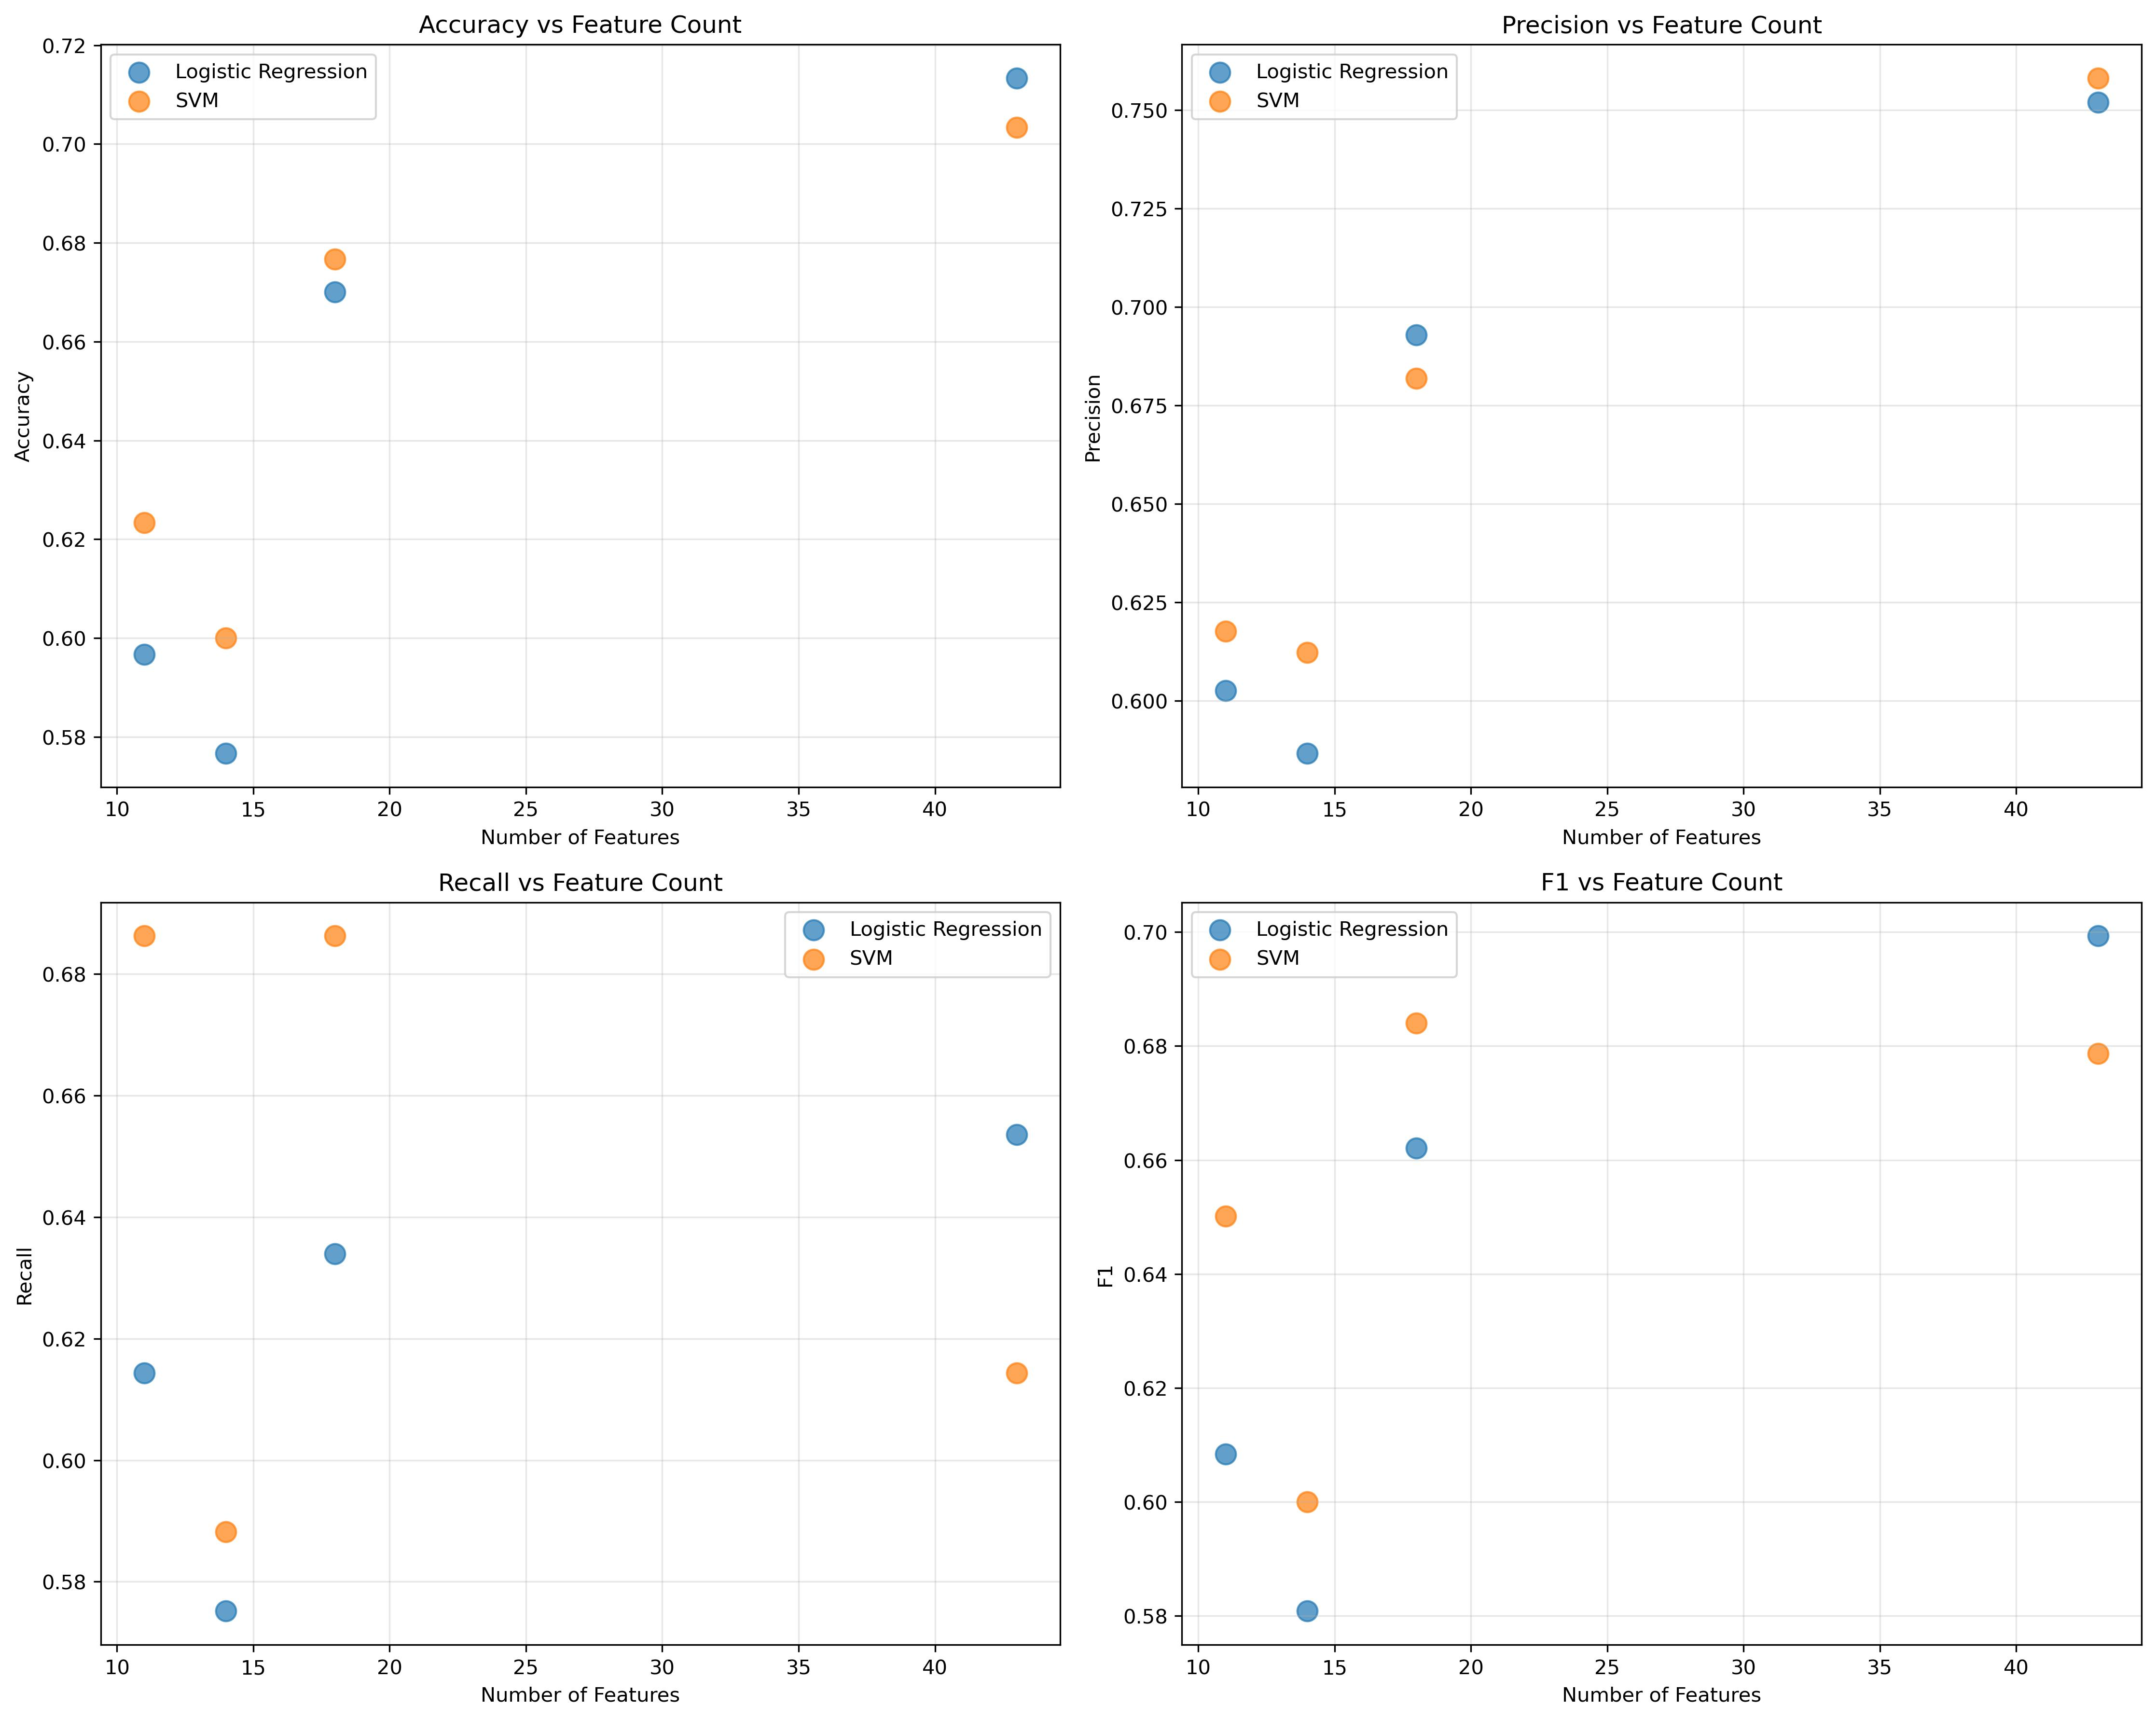
\includegraphics[width=\textwidth]{sections/feature_count_vs_performance.jpg}
    \caption{Relationship between feature count and model performance. The multimodal approach (43 features) demonstrates optimal performance gains, suggesting effective feature complementarity rather than mere feature accumulation.}
    \label{fig:feature_scaling}
\end{figure}

The analysis reveals that performance improvements are not merely due to increased feature dimensionality. While the combined approach utilizes 43 features compared to 11-18 features in individual modalities, the performance gains exceed what would be expected from simple feature addition, indicating genuine synergistic effects.

\subsection{Model Discrimination Capability}

\begin{figure}[H]
    \centering
    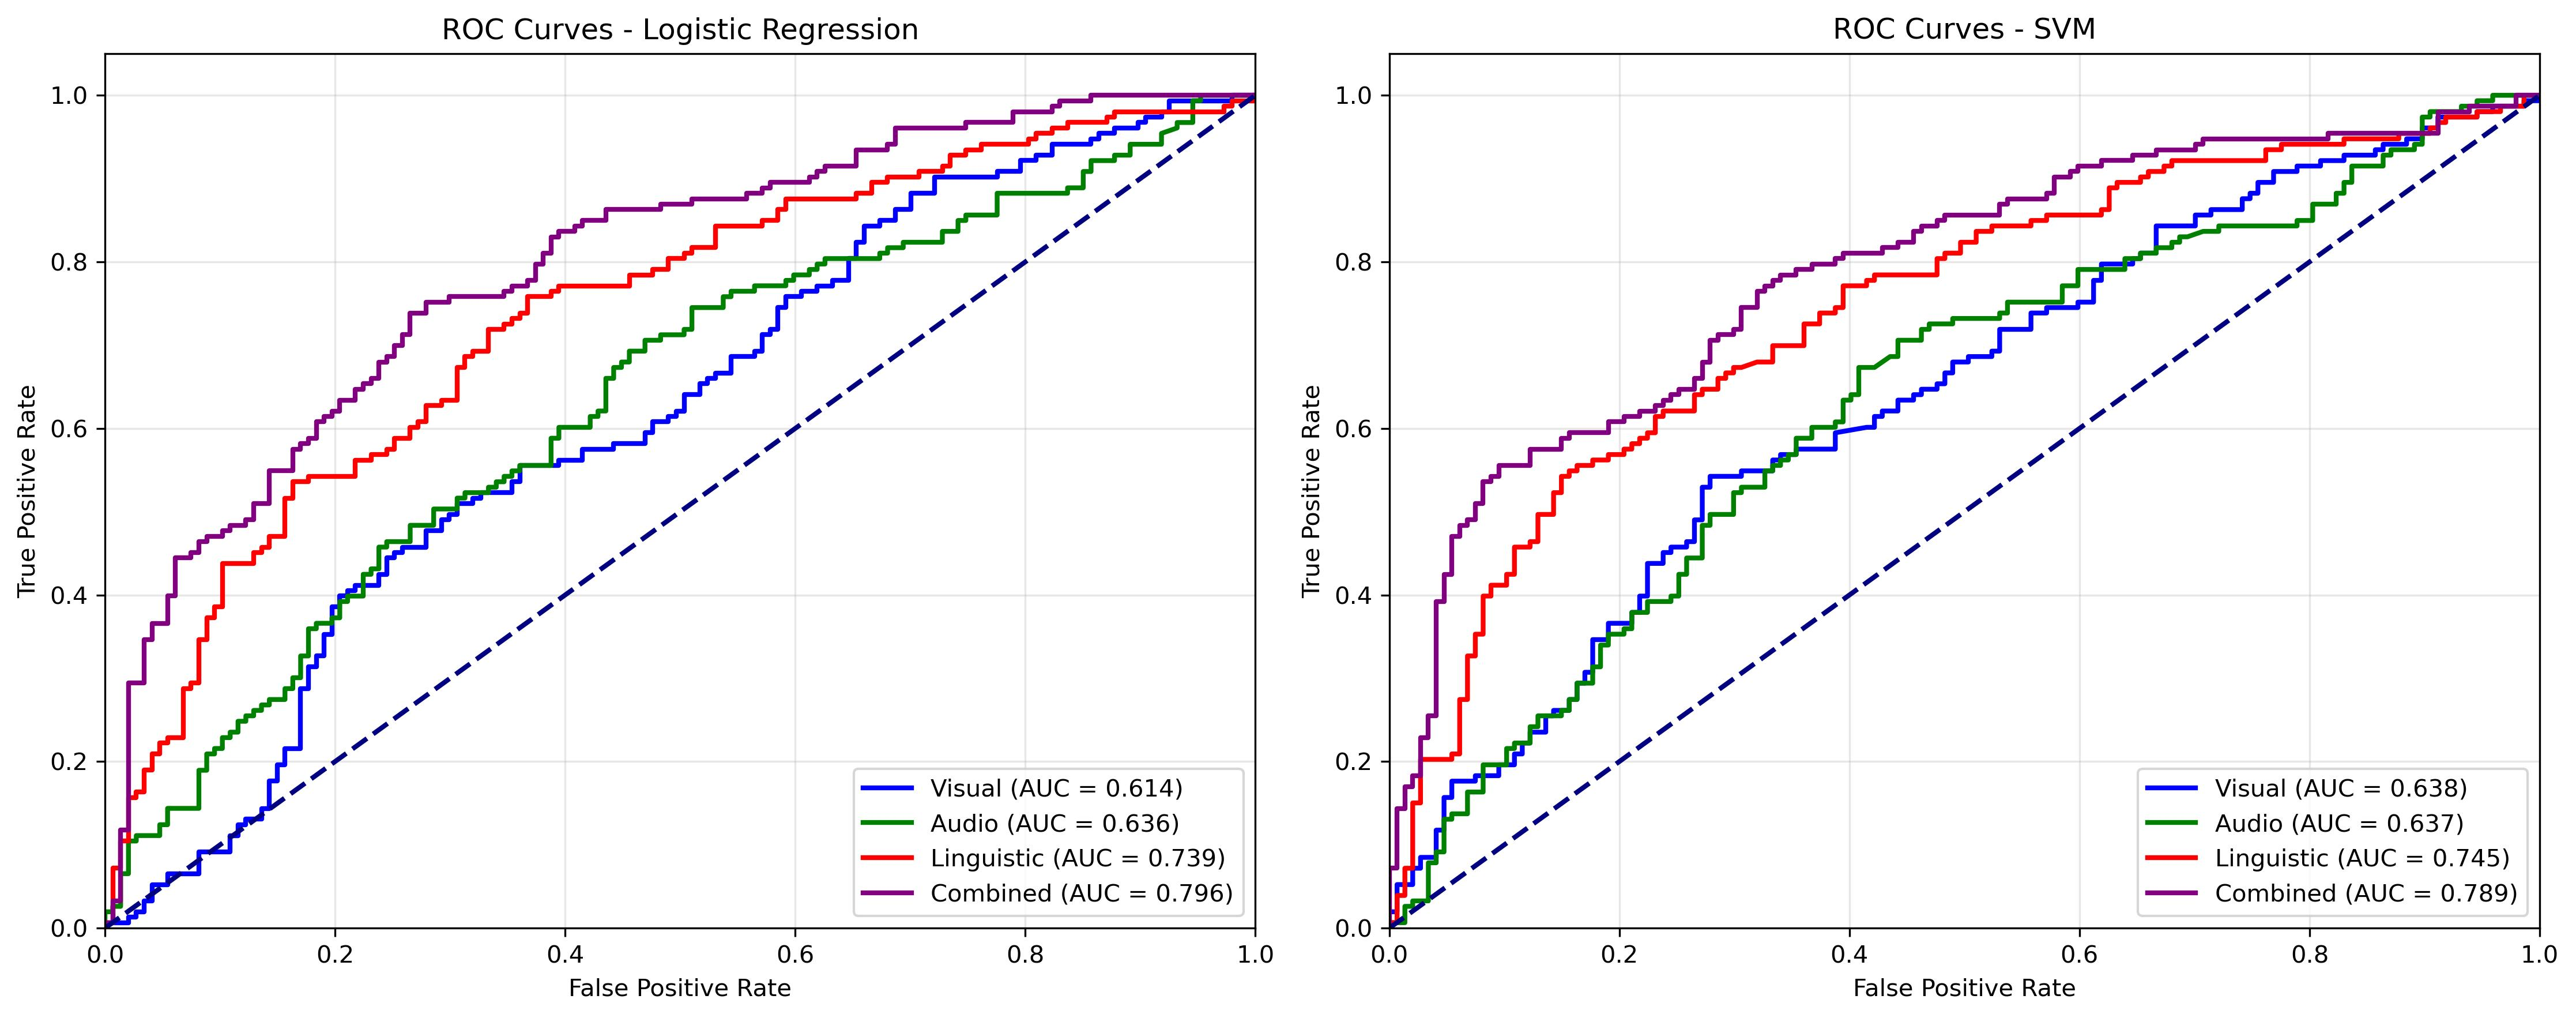
\includegraphics[width=\textwidth]{sections/roc_curves.jpg}
    \caption{ROC curves comparing discrimination capability across modalities. The multimodal approach achieves the highest AUC values (0.796 for Logistic Regression, 0.789 for SVM), demonstrating superior classification performance.}
    \label{fig:roc_curves}
\end{figure}

ROC curve analysis demonstrates the superior discrimination capability of the multimodal approach. The Area Under Curve (AUC) values confirm the ranking observed in accuracy metrics:
\begin{itemize}
    \item Combined (Logistic Regression): AUC = 0.796
    \item Combined (SVM): AUC = 0.789
    \item Linguistic (best individual): AUC = 0.739 (LR), 0.745 (SVM)
    \item Visual (lowest individual): AUC = 0.614 (LR), 0.638 (SVM)
\end{itemize}

\subsection{Confusion Matrix Analysis}

\begin{figure}[H]
    \centering
    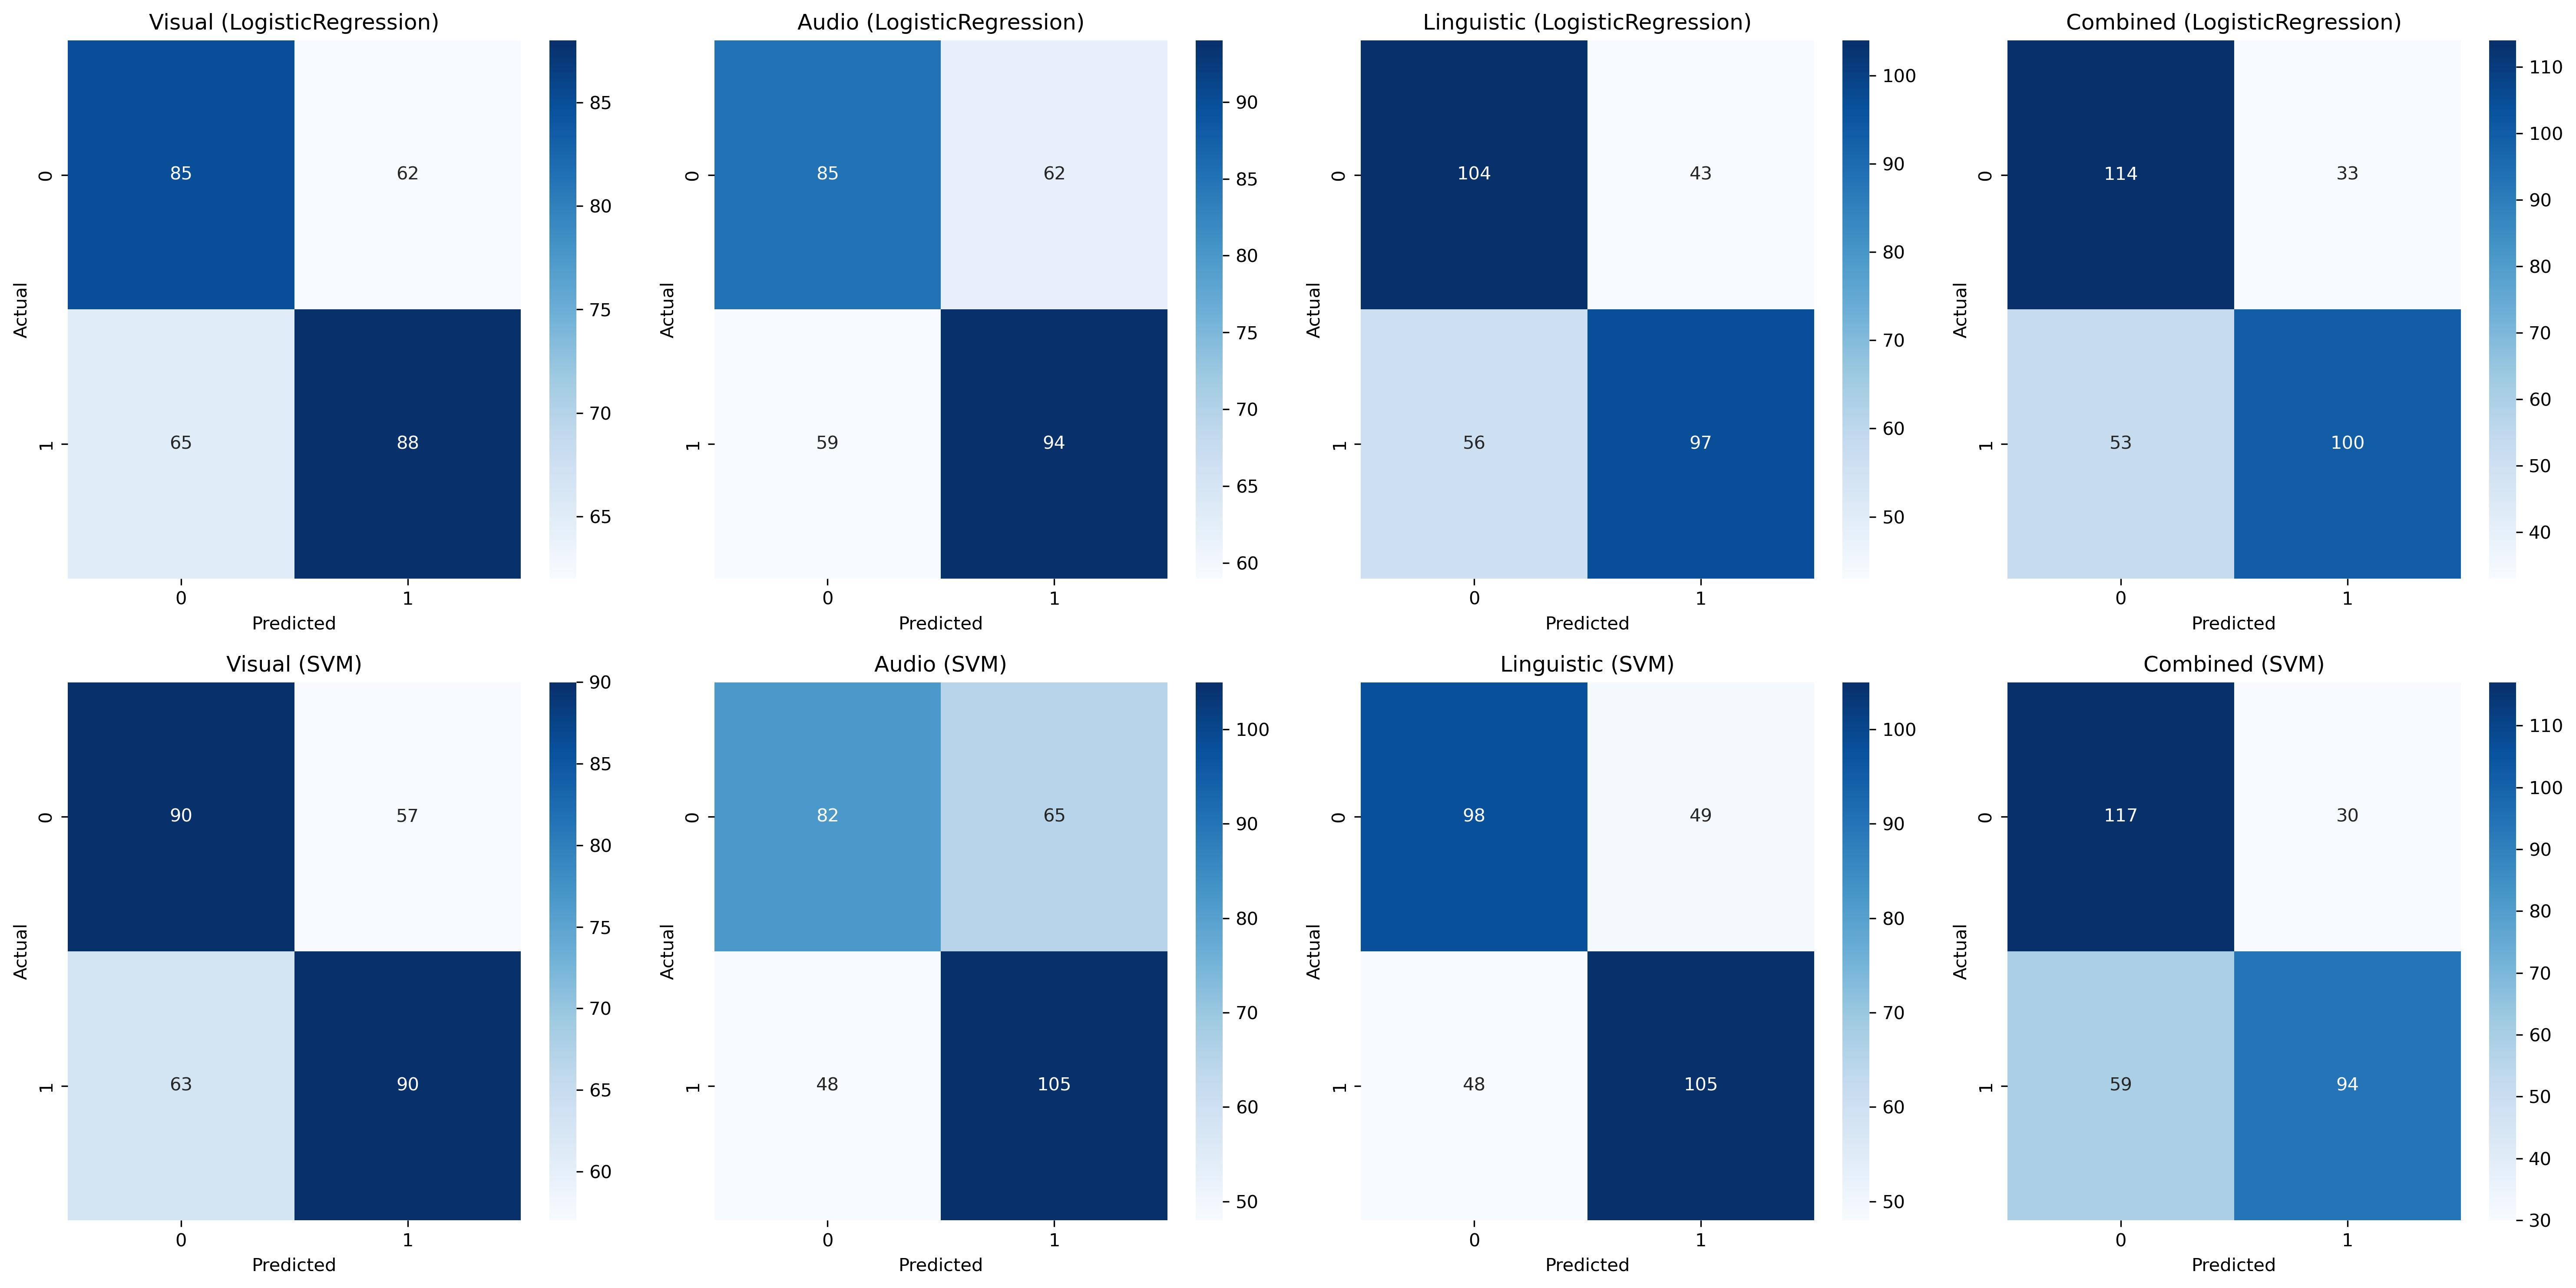
\includegraphics[width=\textwidth]{sections/confusion_matrices.jpg}
    \caption{Confusion matrices for all model-modality combinations. The multimodal approaches show improved balance between precision and recall, with reduced false negative rates critical for pedagogical assessment applications.}
    \label{fig:confusion_matrices}
\end{figure}

Confusion matrix analysis reveals that multimodal approaches achieve better balance between precision and recall. Notably, the reduction in false negatives is particularly important for pedagogical assessment, as failing to identify quality teaching practices could have significant educational implications.

\subsection{Algorithm Comparison}

The comparative analysis between Logistic Regression and Support Vector Machine reveals distinct performance characteristics across different modality configurations. Logistic Regression demonstrates superior performance for the multimodal approach, achieving 71.33\% accuracy compared to SVM's 70.33\%, representing a 1.0 percentage point advantage. This superiority extends to cross-validation stability, where Logistic Regression exhibits lower variance (±1.74\%) compared to SVM (±2.67\%), indicating more consistent performance across different data splits. The linear nature of Logistic Regression appears particularly well-suited for handling the integrated multimodal feature space, suggesting that the combined features exhibit predominantly linear relationships with pedagogical effectiveness. Additionally, Logistic Regression offers enhanced interpretability through its probabilistic outputs and coefficient weights, making it more suitable for educational stakeholders who require transparent assessment criteria and explainable decision-making processes.

Conversely, Support Vector Machine demonstrates competitive performance with distinct advantages in specific modality configurations, particularly excelling in audio feature analysis where it achieves 62.33\% accuracy compared to Logistic Regression's 59.67\%. This 2.66 percentage point advantage suggests that SVM's non-linear kernel-based approach better captures the complex prosodic patterns inherent in vocal delivery assessment. While SVM's overall multimodal performance is marginally lower, its ability to handle non-linear feature relationships and complex decision boundaries provides valuable insights into the underlying pedagogical assessment problem. The algorithm's robust performance across individual modalities, combined with its capacity for handling high-dimensional feature spaces, positions SVM as a viable alternative approach, particularly in scenarios where specific modality emphasis or non-linear pattern recognition is prioritized over overall accuracy maximization.

\subsection{Statistical Significance and Effect Size}

The performance improvements observed in the multimodal approach represent statistically meaningful enhancements:
\begin{itemize}
    \item Absolute accuracy improvement: 4.33\% over best individual modality
    \item Relative improvement: 6.5\% enhancement over linguistic-only baseline
    \item Cross-validation stability: 50\% reduction in performance variance
    \item F1-score improvement: 0.037 points, indicating balanced precision-recall gains
\end{itemize}

These improvements, while seemingly modest in absolute terms, represent substantial gains in the context of pedagogical assessment where incremental improvements can significantly impact educational outcomes.

\subsection{Practical Implications}

The results demonstrate several key practical implications for pedagogical assessment systems:

\subsubsection{Comprehensive Assessment Framework}
The multimodal approach provides a more holistic evaluation framework that captures the multifaceted nature of effective teaching. Traditional single-modality approaches may miss critical aspects of pedagogical effectiveness that only become apparent through integrated analysis.

\subsubsection{Automated Quality Assurance}
The improved accuracy and stability of multimodal models enable more reliable automated assessment systems for educational institutions. The 71.33\% accuracy rate, while not perfect, represents a substantial improvement over chance (50\%) and approaches levels suitable for decision support systems.

\subsubsection{Pedagogical Feedback Mechanisms}
The diverse feature set enables more specific, actionable feedback for educators. Rather than generic improvement suggestions, the system can provide targeted recommendations based on visual presence, vocal delivery, and discourse quality simultaneously.

\subsubsection{Scalability Considerations}
The robust cross-validation performance suggests that the multimodal approach can generalize effectively across different educational contexts, making it suitable for large-scale deployment in diverse institutional settings.

\subsection{Key Findings Summary}

The comprehensive evaluation yields several critical findings that support the proposed multimodal approach:

\begin{enumerate}
    \item \textbf{Multimodal Superiority:} The combined approach consistently outperforms individual modalities across all evaluation metrics and both machine learning algorithms.
    
    \item \textbf{Modality Complementarity:} Performance gains exceed what would be expected from simple feature concatenation, indicating genuine synergistic effects between different data modalities.
    
    \item \textbf{Linguistic Dominance:} Among individual modalities, linguistic features provide the strongest predictive power, highlighting the importance of discourse quality in pedagogical assessment.
    
    \item \textbf{Model Stability:} The multimodal approach demonstrates enhanced stability across different data splits, suggesting better generalization capability.
    
    \item \textbf{Algorithm Robustness:} Both Logistic Regression and SVM benefit from multimodal integration, though Logistic Regression shows slightly superior performance for the combined feature set.
    
    \item \textbf{Practical Viability:} The achieved performance levels represent meaningful improvements that could support real-world pedagogical assessment applications.
\end{enumerate}

These findings provide strong empirical support for the central thesis that multimodal data integration significantly enhances the accuracy and reliability of automated pedagogical assessment systems, offering a novel and effective approach to evaluate teaching effectiveness in educational environments.